\documentclass[a7paper,pagesize,DIV=14,10pt]{scrbook}

\usepackage[french]{babel}
\usepackage[utf8]{inputenc}
\usepackage[T1]{fontenc}
\usepackage{graphicx}
\usepackage{tabularx}
\usepackage{color}
\usepackage{tikz}\usetikzlibrary{shapes.geometric}
\usepackage{url}
\usepackage{import,palatino}
\usepackage{pdfpages,wrapfig,setspace}
\usepackage[left=4mm,right=6mm,top=4mm,bottom=5mm]{geometry}

\setlength{\parskip}{\smallskipamount}
\setlength{\parindent}{0pt}

\begin{document}

\begin{center}
  \textbf{\huge Les algorithmes}
  
  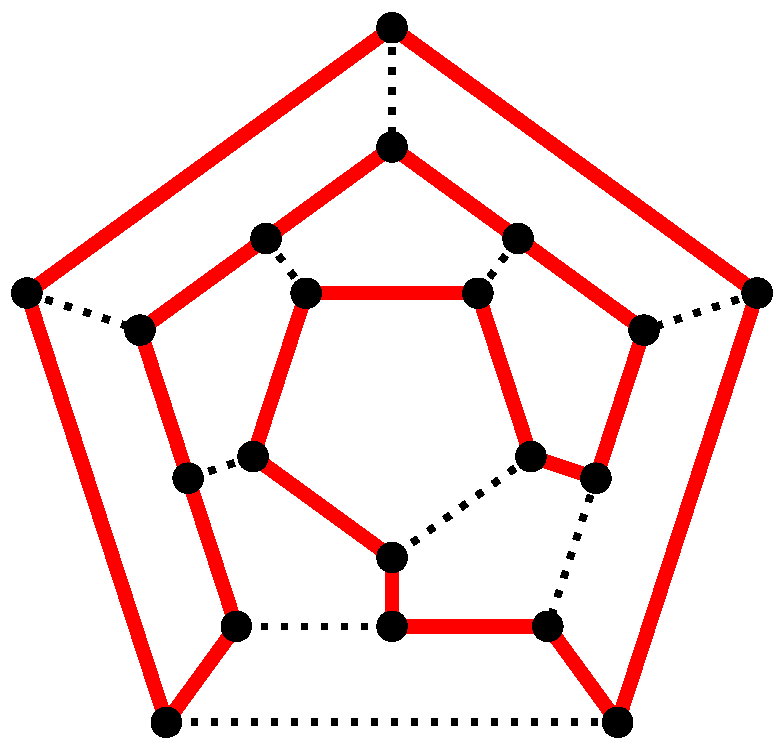
\includegraphics[width=.5\linewidth]{img/Hamiltonian_path.pdf}
\end{center}

\vspace{-.5\baselineskip} %
Ce livret contient 3 activités débranchées pour explorer la base de
l'informatique

\medskip
\centerline{\large\textit{Qu'est ce qu'un algorithme?}}

\bigskip
\centerline{  
\includegraphics[width=.9\linewidth]{img/logo_SMN.pdf}}


\begin{minipage}{.8\linewidth}
  \begin{spacing}{.5}
    \hbox to \linewidth{\tiny~\hfill Vous pouvez copier, modifier et diffuser librement ce document,}
    \hbox to \linewidth{\tiny~\hfill à condition de laisser ces mêmes droits à vos lecteurs.}
  \end{spacing}
\end{minipage}%
~
\begin{minipage}[b]{.16\linewidth}
  
\includegraphics[width=\linewidth]{img/logo_by-sa.pdf}
\end{minipage}%


%%%%%%%%%%%%%%%%%%%%%%%%%%%%%%%%%%%%%%%%%%%%%%%%%%%%%%%%%%%%%%%%%%%%%%%%%%%%
%%%%%%%%%%%%%%%%%%%%%%%%%%%%%%%%%%%%%%%%%%%%%%%%%%%%%%%%%%%%%%%%%%%%%%%%%%%%
%%%%%%%%%%%%%%%%%%%%%%%%%%%%%%%%%%%%%%%%%%%%%%%%%%%%%%%%%%%%%%%%%%%%%%%%%%%%
\section*{Le jeu de Nim}

\vspace{-.5\baselineskip}
Ce premier jeu se joue à deux joueurs.\\
On dispose de 16 objets quelconques.\\
Chacun à son tour prend 1, 2 ou 3 objets.\\
\textbf{But du jeu:} prendre le dernier.

\vspace{-.5\baselineskip}
\subsubsection*{Un algorithme pour gagner}

\vspace{-.5\baselineskip} %
Le joueur n$^o$2 a une \textbf{stratégie gagnante} infaillible: il
s'assure de laisser 12, 8 puis 4 objets à son adversaire.

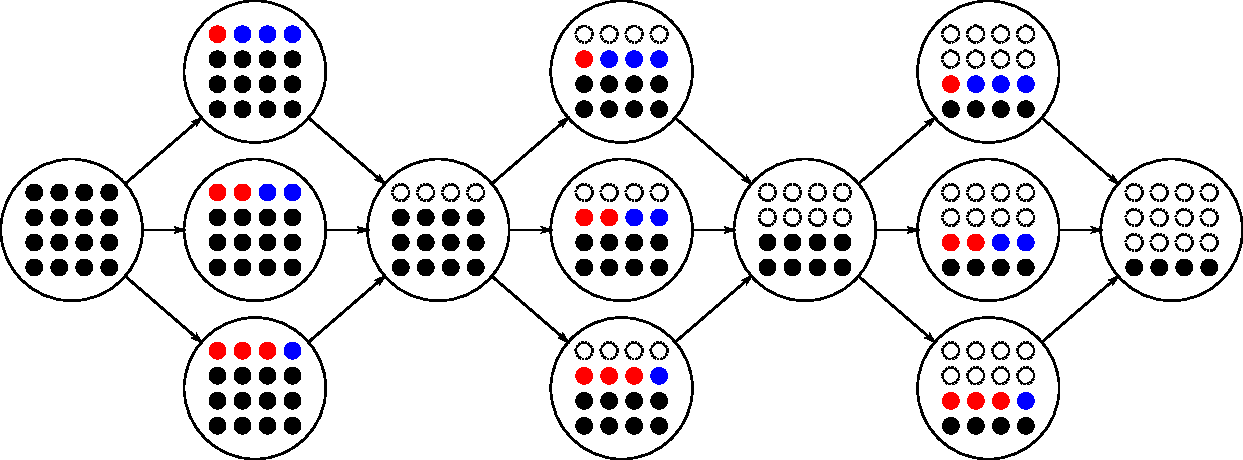
\includegraphics[width=\linewidth]{img/nim16.pdf}

\subsection*{C'est de l'informatique}
\vspace{-.5\baselineskip} %
Les algorithmes sont très importants pour assurer que l'ordinateur
fasse \textbf{à coup sûr} ce que l'on attend de lui.

\newpage
%%%%%%%%%%%%%%%%%%%%%%%%%%%%%%%%%%%%%%%%%%%%%%%%%%%%%%%%%%%%%%%%%%%%%%%%%%%%
%%%%%%%%%%%%%%%%%%%%%%%%%%%%%%%%%%%%%%%%%%%%%%%%%%%%%%%%%%%%%%%%%%%%%%%%%%%%
%%%%%%%%%%%%%%%%%%%%%%%%%%%%%%%%%%%%%%%%%%%%%%%%%%%%%%%%%%%%%%%%%%%%%%%%%%%%
\section*{Le crêpier psycho-rigide}

\vspace{-.5\baselineskip}
Les planchettes sont des crêpes, qu'il faut ranger de la plus grande à
la plus petite.

\smallskip
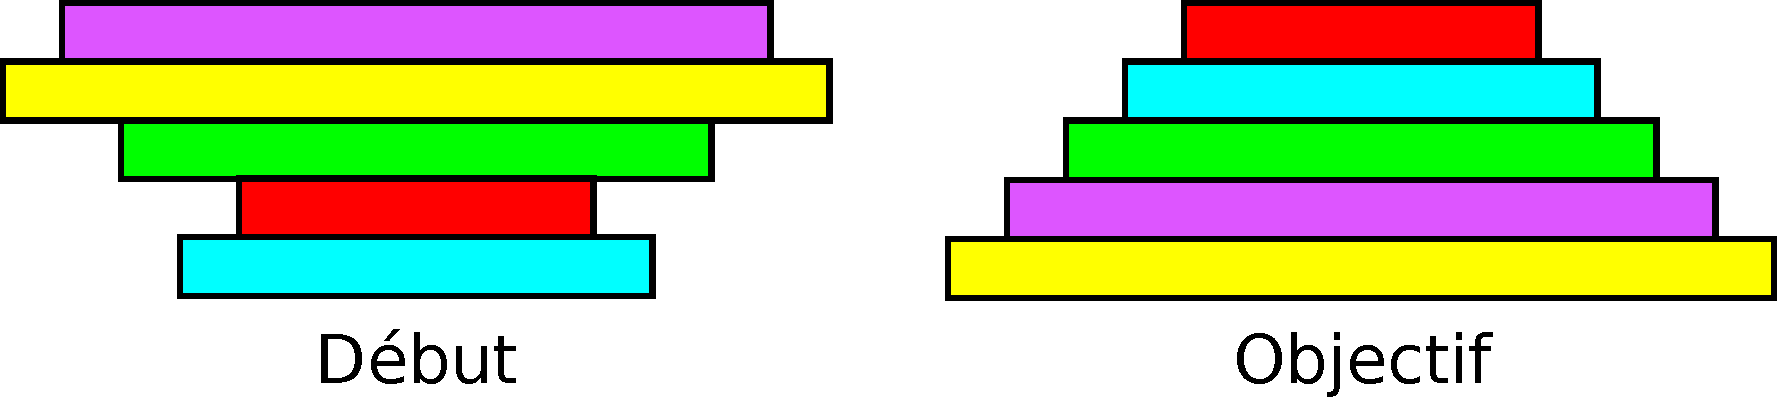
\includegraphics[width=\linewidth]{img/crepes_but-du-jeu.pdf}

À chaque coup, on retourne le haut de la pile (une ou plusieurs crêpes,
d'un bloc).

\smallskip
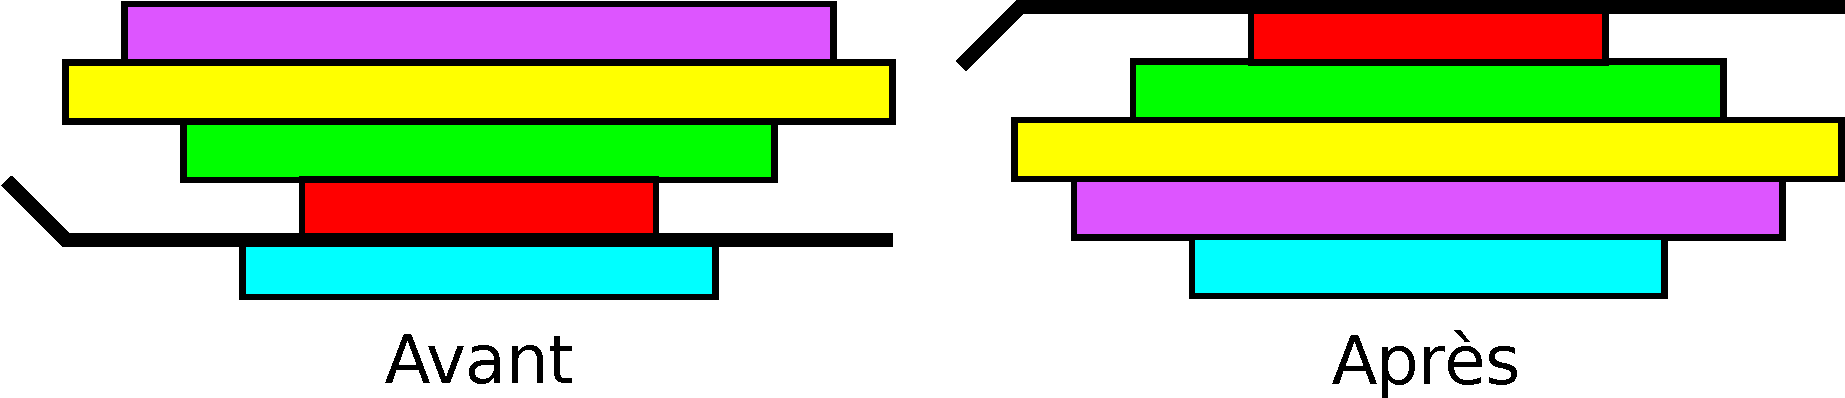
\includegraphics[width=\linewidth]{img/crepes_un-coup.pdf}

\medskip%
On n'a pas le droit de poser des crêpes à coté, ni de soulever celles
du haut pour changer celles au milieu de la pile.

\bigskip%
\textbf{Variante} (plus dure): il faut en plus que la face colorée des
crêpes soit visible.

\newpage
\subsection*{Trouver l'algorithme du crêpier}
\vspace{-.5\baselineskip}

Il faut se fixer des objectifs intermédiaires. Par exemple, placer la
plus grand crêpe tout en bas puis ne plus y toucher.

\smallskip
Est-ce qu'il y a une situation où je sais amener la grande crêpe tout en bas?

\smallskip
Comment faire pour me ramener dans cette situation où je sais ranger la grande crêpe?

\subsection*{C'est de l'informatique}
\vspace{-.5\baselineskip}

Un algorithme, ce n'est pas forcément compliqué. Tout le monde peut en découvrir.

\smallskip
Un ordinateur est très obéissant: il lui faut des instructions
précises et sans ambiguïté.

\vspace{-.5\baselineskip}
\subsection*{Aller plus loin}
\vspace{-.5\baselineskip}
D'autres algorithmes existent pour ce problème. On peut les programmer
avec la PLM, l'\textit{exerciseur de l'apprenti programmeur}.\\
{\small\color{blue}\url{http://www.loria.fr/~quinson/PLM/}}

\newpage
%%%%%%%%%%%%%%%%%%%%%%%%%%%%%%%%%%%%%%%%%%%%%%%%%%%%%%%%%%%%%%%%%%%%%%%%%%%%
%%%%%%%%%%%%%%%%%%%%%%%%%%%%%%%%%%%%%%%%%%%%%%%%%%%%%%%%%%%%%%%%%%%%%%%%%%%%
%%%%%%%%%%%%%%%%%%%%%%%%%%%%%%%%%%%%%%%%%%%%%%%%%%%%%%%%%%%%%%%%%%%%%%%%%%%%
\section*{Le baseball multicolore}

\newcommand{\maisonPair}[5]{ 
  \node[name=#1 m,at=(#1.base),shape=regular polygon,thin,regular polygon sides=#3,minimum size=8.5mm,rotate=(360/#3)] {};
  \node[name=#1 b,at=(#1.base),shape=regular polygon,thin,regular polygon sides=#4,minimum size=15mm,rotate=(360/#4)/2]{};
  \foreach \base/\maison in {#5} {
    \draw[shift=(#1 m.corner \base)]
       node[shape=ellipse,fill=\maison,draw=black,thin,rotate=((360/#3)*(\base-1))+(360/#3/2)]
           {~~~};
  }
  \foreach \bb in {1,...,#4} {
    \draw[shift=(#1 b.corner \bb)] node[name=bb \bb]{};
  }
  \foreach \base/\maison in {#2} {
    \draw[shift=(#1 b.corner \base)]
       node[name=bb \base,shape=circle,fill=\maison,thin,draw=\maison,inner sep=.1]
           {~~~};
  }
}


\newcommand{\maisonImpair}[5]{ \begin{tikzpicture}
  \node[name=maison,shape=regular polygon,regular polygon sides=#3,minimum size=18mm, inner sep=0pt]{};
  \node[name=base,shape=regular polygon,regular polygon sides=#4,minimum size=12mm]{};
  \foreach \base/\maison in {#5} {
    \draw[shift=(maison.corner \base)]
       node[shape=ellipse,fill=\maison,draw=black,rotate=(360/#3)*(\base-1),name=m \base] {~~~~~};
  }
  \foreach \base/\maison in {#1} {
    \draw[shift=(base.corner \base)]
       node[shape=circle,fill=\maison,draw=black,inner sep=.1] {~~~};
  }
  \foreach \bb in {1,...,#4} {\draw[shift=(b.corner \bb)] node[name=bb \bb] {};}



%  \foreach \bb in {1,...,#4} {\draw[shift=(b.corner \bb)] node[name=bb \bb]{\tiny\bb};}%debug the bonshommes names
  #2
\end{tikzpicture} }

\newcommand{\maisonQuatre}[2]{\maisonPair{#1}{#2}{4}{12}{1/A,2/B,3/C,4/D}}
\newcommand{\maisonCinq}[2]{\maisonImpair{#1}{#2}{5}{20}{1/A,2/B,3/C,4/D,5/E}}
\newcommand{\maisonSix}[2]{\maisonPair{#1}{#2}{6}{24}{1/A,2/B,3/C,4/D,5/E,6/F}}
\newcommand{\maisonSept}[2]{\maisonImpair{#1}{#2}{7}{28}{1/A,2/B,3/C,4/D,5/E,6/F,7/G}}

\colorlet{A}{green!60}
\colorlet{B}{red!80}
\colorlet{C}{purple!40}
\colorlet{D}{black!2!yellow}
\colorlet{E}{blue!70}
\colorlet{F}{orange!80}
\colorlet{G}{olive}
\colorlet{H}{magenta}
\colorlet{I}{lime}
\colorlet{J}{pink}
\colorlet{Z}{white}

\newcommand{\Pawn}[1]{\node[shape=circle,fill=#1,draw=black,inner sep=.1] {~~~}}
\newcommand{\pawn}[1]{\tikz \draw node[shape=circle,fill=#1,draw=black,inner sep=.1] {~~~};}



\vspace{-.5\baselineskip} %
Plusieurs bases sont disposées en cercle.  Il y a deux pions par base,
sauf une couleur avec un seul pion et un emplacement vide.  Chaque
pion veut rejoindre sa base.

%\vspace{-.5\baselineskip}
\begin{minipage}{.5\linewidth}\center
  \maisonCinq{1/A,2/B, 5/E,6/C,   9/D, 13/B,14/A, 17/C,18/D} {}

 \textbf{Situation initiale} 
\end{minipage}~
\begin{minipage}{.5\linewidth}\center
  \maisonCinq{1/A,2/A, 5/B,6/B, 9/C,10/C, 13/D,14/D, 17/E}{}

  \textbf{Situation finale}
\end{minipage}

À chaque coup, l'emplacement vide est occupé par un pion d'une
\textbf{base voisine}, sans traverser le terrain. On n'échange pas
entre deux bases pleines.

\begin{minipage}{.5\linewidth}\center
  \maisonCinq{1/A,2/B, 5/E,6/C,   9/D, 13/B,14/A, 17/C,18/D}
             {
                  \draw[->,ultra thick,draw=black!10!green] (bb 5) .. controls (0pt,0pt).. (bb 10);
                  \draw[->,ultra thick,draw=black!10!green] (bb 6) .. controls (0pt,0pt).. (bb 10);
                  \draw[->,ultra thick,draw=black!10!green] (bb 13) .. controls (0pt,0pt).. (bb 10);
                  \draw[->,ultra thick,draw=black!10!green] (bb 14) .. controls (0pt,0pt).. (bb 10);}

  \textbf{Coups autorisés}
\end{minipage}~\begin{minipage}{.5\linewidth}\center
  \maisonCinq{1/A,2/B, 5/E,6/C,   9/D, 13/B,14/A, 17/C,18/D}{
    % Des marqueurs pour faire des fleches en rond
    \node[name=c,shape=regular polygon,regular polygon sides=5,rotate=72*4,minimum size=12mm]{};
    \foreach \cc in {1,...,5} {\draw[shift=(c.corner \cc)] node[name=cc \cc] {};}

    \draw[<->,ultra thick,draw=red,bend left=45] (cc 1) -- (cc 2);
    \draw[<->,ultra thick,draw=red,bend left=45] (cc 2) -- (cc 3);
    \draw[<->,ultra thick,draw=red,bend left=45] (cc 5) -- (cc 1);

    \draw[<->,ultra thick,draw=red,bend left=45] (cc 3) -- (cc 1);
    \draw[<->,ultra thick,draw=red,bend left=45] (cc 2) -- (cc 5);
    \draw[<->,ultra thick,draw=red,bend left=45] (cc 1) -- (cc 4);
    \draw[<->,ultra thick,draw=red,bend left=45] (cc 4) -- (cc 2);
                }

  \textbf{Coups interdits}
\end{minipage}

\newpage ~\vfill \centerline{(page 6 vide pour l'instant)} \vfill

\newpage ~\vfill \centerline{(page 7 vide pour l'instant)} \vfill
\newpage ~\vfill \centerline{(page 8 vide pour l'instant)} \vfill

\end{document}
